\section{Exercise 1b}
\lstinputlisting{downhill.py}
\lstinputlisting{Ex1b.py}

For the second subquestion, we have to fit the model to some data using a $\chi^2$ method. Firstly, the data is divided into 100 bins ranging from $10^{-4}$ to 5 in log space. To normalize them, we divide the bins by the number of halos taken from each file. The next step is to minimize the log-likelihood of the $\chi^2$. The negative log-likelihood is given by the following equation: 
\begin{equation}
    -\ln{L} = \sum^{N_b-1}_{i = 0} \left[ \frac{1}{2} \ln(2\pi\sigma_i^2) +\frac{1}{2}\frac{[y_i - y(x_i|a,b,c)]^2}{\sigma_i^2}  \right]
\end{equation}

In our case, we can ignore the first part for minimizing, because it is constant as long as $\sigma_i^2 \neq \sigma_i^2(\textbf{p})$, which is the case. Furthermore, $y_i$ are the bin values and $y(x_i|a,b,c) = \sigma_i^2 = \tilde{N} = 4\pi\int^{x_i+1}_{x_i} n(x) x^2 dx$. This is the integral of the model over every bin. In order to make the code more efficient, I made an adjustment to my Romberg algorithm of the previous assignment. The new algorithm is able to calculate the integral of a function for multiple lower and upper limits at the same time. This decreased the calculation time significantly. The code is shown in the appendix. The log-likelihood is minimized using a downhill-simplex algorithm (quicksort also shown in appendix). For every new step in the downhill-simplex, the model has to be normalized again. Therefore, we calculate A for every step. When the target is reached, the best points a, b and c are returned, just as the lowest likelihood. The results of the $\chi^2$ are. Some of the likelihoods are very high, which might indicate the fit is not very good. 
\\
\\
\lstinputlisting{Ex1b.txt}


The results are shown in the Figure below.

\begin{figure}[h!]
  \centering
  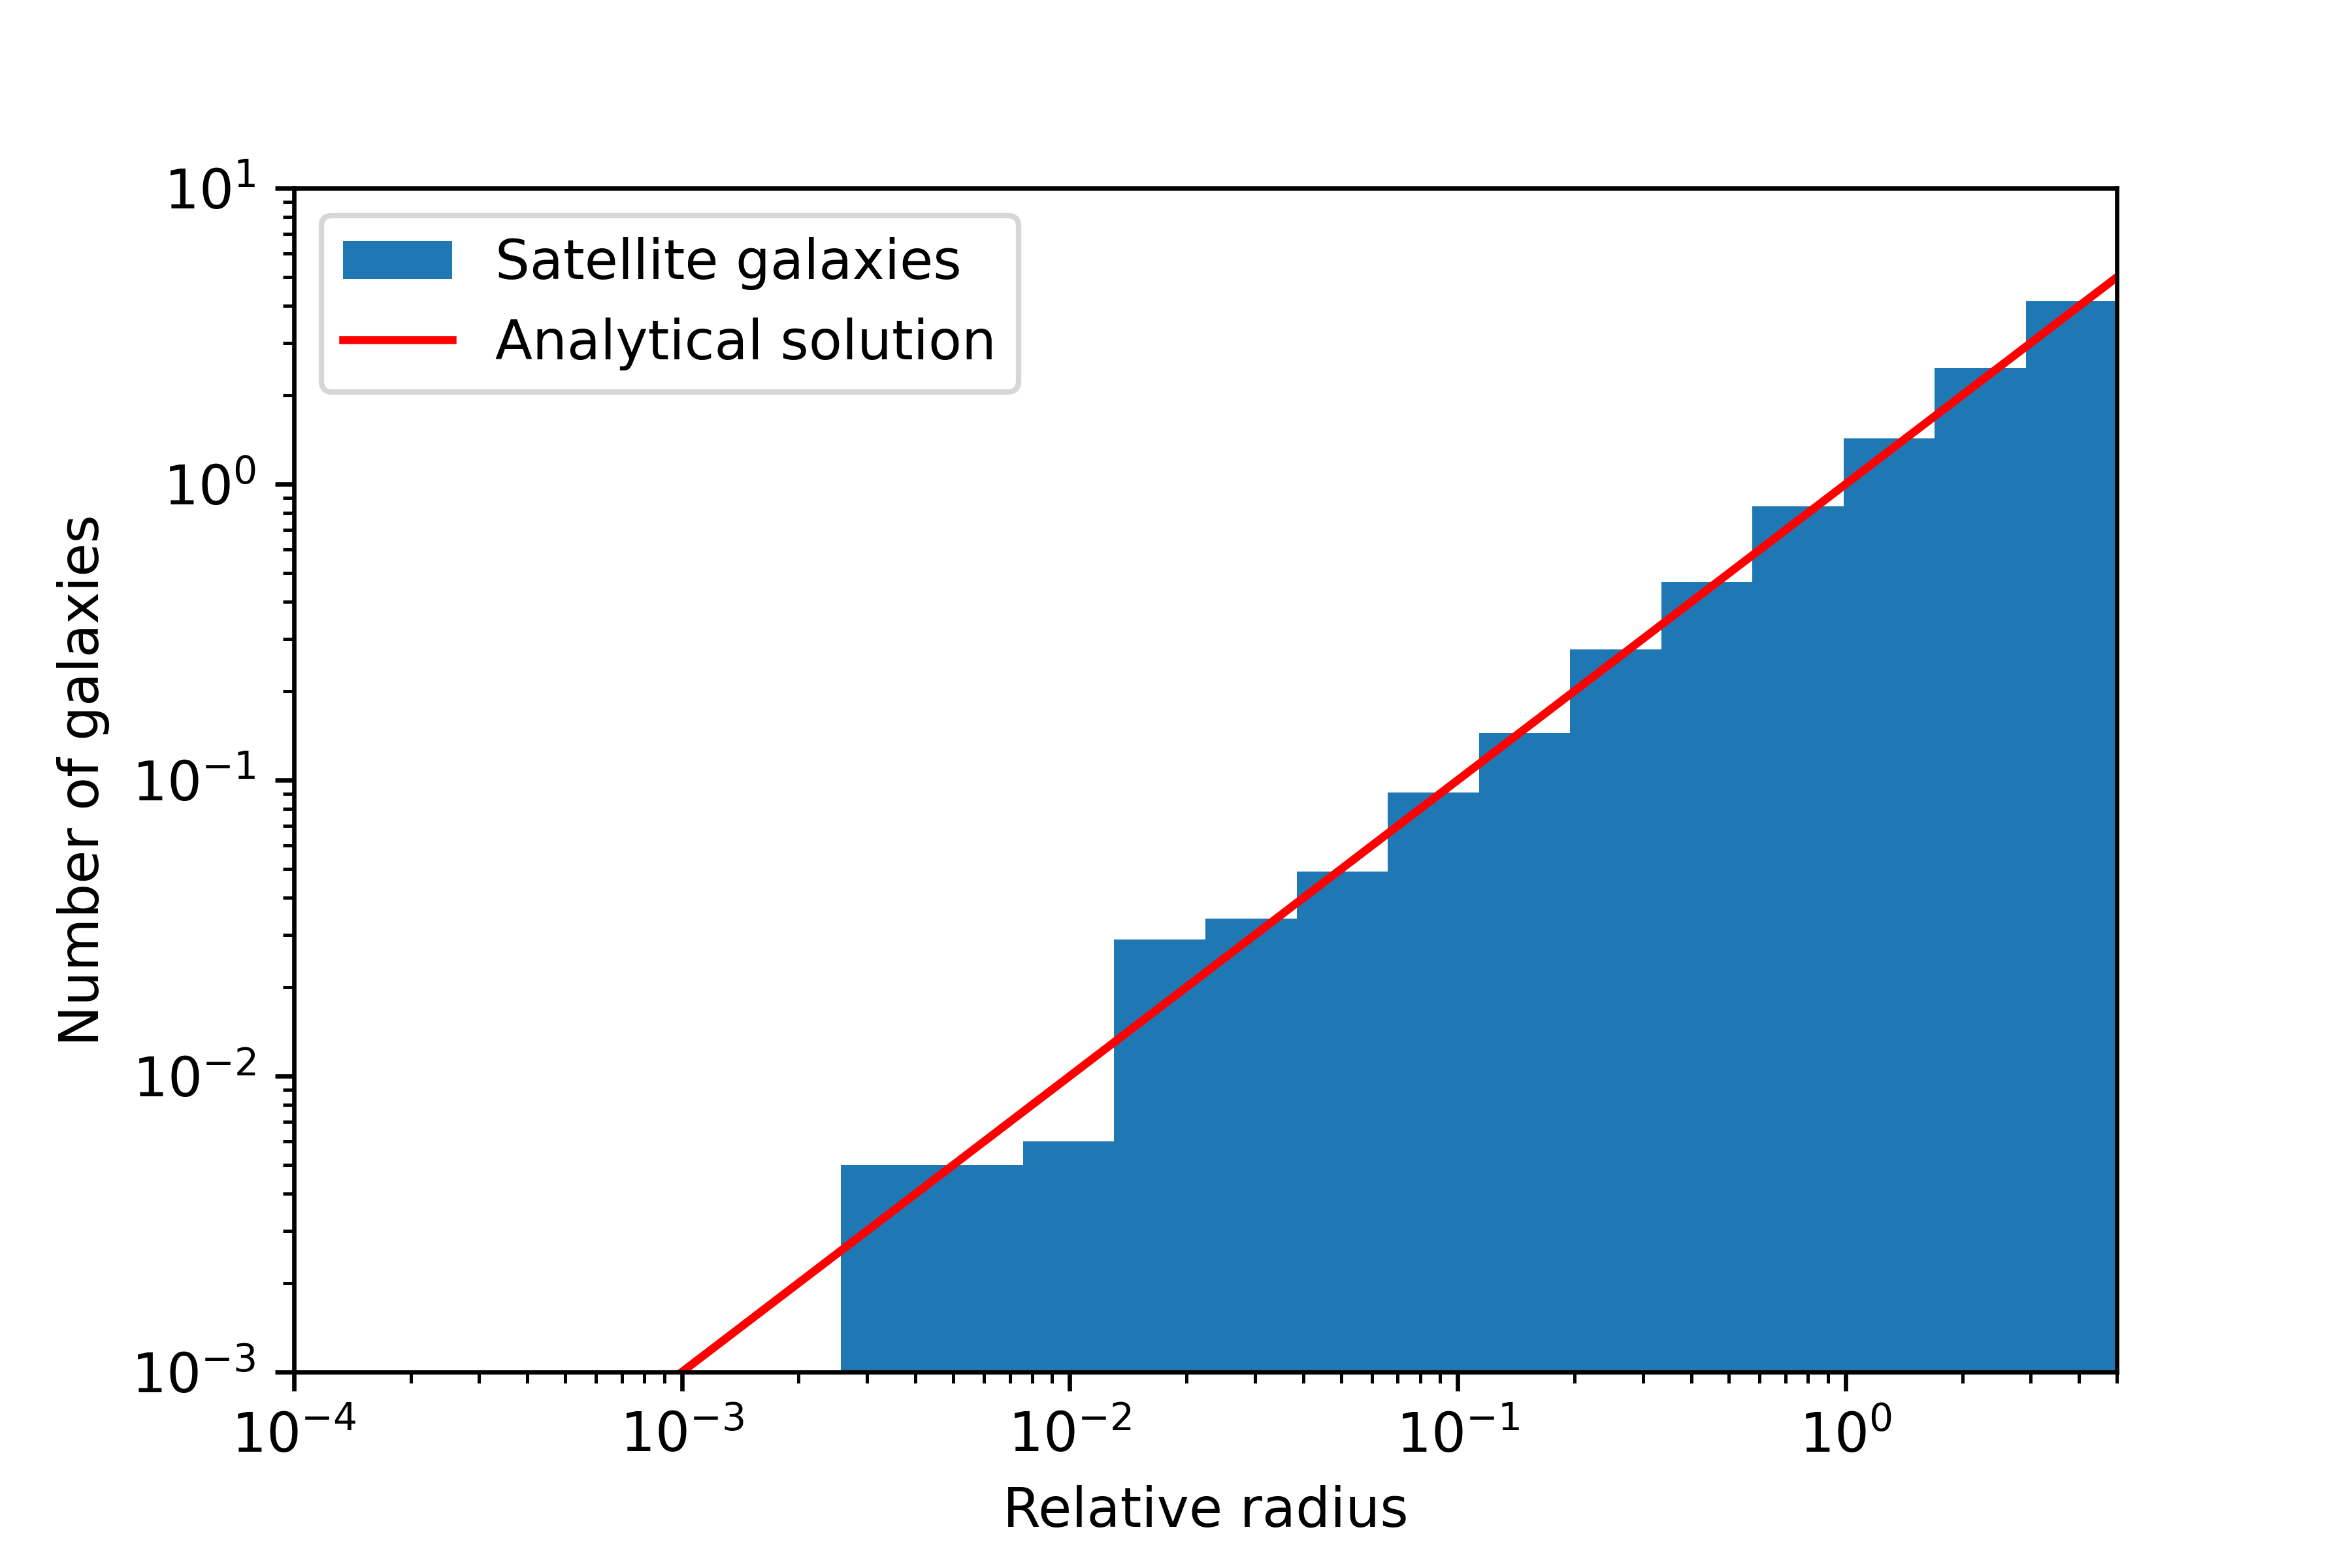
\includegraphics[width=0.9\linewidth]{my_solution_1b.png}
  \caption{A $\chi^2$ fit to the data. In the figure, it seems like the fitted model is overestimating at low radii. This might be due to the low number of satellites with a low radius.}
\end{figure}


